\chapter{Conclusiones} \label{chp:impacto}

%%%%%%%%%%%%%%%%%%%%%%%%%%%%%%%%%%%%%%%%%%%%%%%%%%%%%%%%%%%%%%%%%%%%%%%%%%%%%%%%
%%%%%%%%%%%%%%%%%%%%%%%%%%%%%%%%%%%%%%%%%%%%%%%%%%%%%%%%%%%%%%%%%%%%%%%%%%%%%%%%

\section{Evaluación de objetivos}

La presente sección tiene como finalidad valorar el grado de cumplimiento de los objetivos definidos al inicio de este Trabajo Fin de Grado. El objetivo general consistía en desarrollar una metodología integral para el análisis topológico y estadístico de trayectorias en espacios de baja y alta dimensión, permitiendo extraer información relevante para su interpretación y clasificación. Para lograrlo, se establecieron una serie de objetivos específicos que han guiado el desarrollo del proyecto y que, en su conjunto, han sido abordados satisfactoriamente.

En primer lugar, se ha llevado a cabo una correcta definición y documentación del problema, delimitando las variables relevantes para el estudio de trayectorias en contextos tanto físicos como abstractos. Esta tarea incluyó la selección del conjunto de datos (GeoLife), la identificación de los atributos espaciales y temporales clave y la representación de las trayectorias en forma de nubes de puntos tridimensionales, preparadas para su análisis mediante herramientas topológicas.

A continuación, se diseñó una metodología de análisis que integró con éxito técnicas de Análisis Topológico de Datos (TDA) como la homología persistente y el algoritmo Mapper, junto con métodos estadísticos tradicionales y algoritmos de agrupamiento. Este diseño metodológico permitió identificar patrones estructurales en los datos, tales como bucles, componentes conexas y trayectorias atípicas, aportando una perspectiva más rica que la proporcionada por enfoques puramente estadísticos.

La implementación de la propuesta se realizó utilizando un conjunto de herramientas en el lenguaje Python, incluyendo librerías especializadas como Giotto-TDA, Scikit-learn y Pandas. Esta implementación fue puesta a prueba mediante diversos experimentos que validaron la eficacia de la metodología propuesta. Se evaluaron aspectos como la robustez frente al ruido, la sensibilidad ante anomalías y la eficiencia computacional, especialmente al aplicar técnicas de paralelización para mejorar los tiempos de ejecución.

Finalmente, los resultados fueron interpretados y sintetizados de forma rigurosa. Se analizaron las estructuras topológicas detectadas en los datos, se compararon con los resultados obtenidos por métodos tradicionales como PCA y clustering, y se discutieron las implicaciones prácticas del enfoque propuesto. 

Esta evaluación permitió extraer conclusiones relevantes para el campo del análisis de trayectorias, destacando las ventajas del uso de TDA frente a técnicas convencionales y proponiendo líneas futuras de investigación orientadas a su integración con modelos de aprendizaje profundo.

En resumen, los objetivos planteados en este trabajo han sido cumplidos de manera sólida, evidenciando la utilidad del enfoque topológico-estadístico en el análisis de trayectorias y demostrando su potencial para aplicaciones en movilidad, sistemas dinámicos y análisis de datos complejos.


\section{Trabajo futuro} \label{sct:resultados_trabajofuturo}

Este proyecto nos ofrece una visión relativamente limitada de la potencia que poseen las herramientas de análisis especificas para TDA, al no tener a disposición ni el tiempo ni los recursos computacionales que harian falta para una investigación más en detalle. Se podrían abrir varias líneas de investigaciones relativas a una variedad de factores, ya sea los factores relativos al uso de recursos computacionales, aquellos relativos a los datos usados, etc.

En primer lugar, desde el punto de vista de la mayor explotación de la potencia de las herramientas de análisis, se plantearía el uso de otras herramientas o librerías especificas de TDA, ya sea haciendo uso de otras funciones disponibles dentro de la propia librería \textit{giotto-tda}, o haciendo uso de alternativas como las mencionadas en la sección \ref{Herramientas} del capítulo de estado del arte. Adicionalmente, se podría hacer uso de volúmenes de datos mayores, aprovechando la capacidad de integración de la librerías de análisis con multi-threading, ya sea haciendo uso de recursos computacionales para alto rendimiento en servicios en la nube, o solicitando el uso de súper computadores como podría ser el Magerit-3.

En segundo lugar, el proyecto se podría expandir modificando los datos que son objetos del análisis, ya que el uso de otro tipo de trayectorias físicas o del mundo real, como podría ser el uso de datos médicos, o plantear alternativas basadas en fenómenos más abstractos, como podrían ser los atractores caóticos o espacios fuera de métricas tradicionales como sería la euclidiana, podrían abrir líneas de desarrollo que podrían generar bastante interés. 

Partiendo de la idea de modificar los datos, se podrían hace ligeras transformaciones a las trayectorias usadas actualmente para ver la evolución de las características topológicas de las mismas, por ejemplo, aplicando desplzamientos, o lag, en ciertos intervalos de los datos, generando conjuntos de datos de mayor dimensionalidad, que revelan la depedencia espacial y temporal, y la oportunidad de analizar no solamente la naturaleza de los datos, sino también su robustez ante estos cambios.

Finalmente, se podría expandir el proyecto haciendo uso de soluciones híbridas, implementando las herramientas de clusterizacion y análisis habitualmente usadas en machine learning y análisis de datos, y combinándolas con las soluciones de TDA para poder un análisis mas completo, que nos ofrece una visión más global de las características de un determinado conjunto de datos.

\section{Conclusiones personales} \label{sct:resultados_conclusiones}

La realización de este Trabajo de Fin de Grado ha supuesto un hito de gran valor, tanto en lo académico como en lo personal. Durante el proceso de realización del mismo, he tenido la oportunidad de adentrarme en el campo del Análisis Topológico de Datos (TDA), una disciplina que, si bien requiere de una base matemática sólida para entender algunos de los conceptos clave de la misma, con conocimientos básicos de programación, se nos ofrece un conjunto de herramientas muy potentes para el estudio de estructuras de datos no triviales, como lo son las trayectorias espaciales, que nos permiten realizar análisis de una complejidad considerable, ofreciéndonos una alternativa más optimizada respecto las que nos darían los métodos de análisis tradicional.

A lo hora de ejecutar con una sola trayectoria, se seleccionó una trayectoria de complejidad media, de alrededor de 90 puntos, todos en intervalos de tiempo consecutivos

En lo relativo a los conocimientos técnicos, este proyecto me ha permitido consolidar conocimientos en programación científica y herramientas de análisis de datos con Python, especialmente en el uso de bibliotecas especializadas como \texttt{giotto-tda}, \texttt{scikit-learn}, \texttt{matplotlib} y \texttt{pandas}, siendo algunas de estas herramientas de uso común el mercado profesional. También he mejorado mis conocimientos y he ganado experiencia a la hora de manipular conjuntos de datos reales de tamaño considerable (como el dataset de trayectorias \textit{Geolife}), en la depuración de  problemas relacionados con formatos de datasets y limpieza y transformación a conjunto de datos, en la evaluación de necesidad de cómputo y la optimización del rendimiento computacional con herramientas de software, y a gestionar entornos mixtos de desarrollo, tanto en local como en la nube, mediante Google Colab.

Desde el punto de vista metodológico, ha sido muy enriquecedor explorar la comparación entre métodos tradicionales como serian PCA, k-means, DBSC, entre otros, y métodos topológicos, como la homología persistente y el algoritmo Mapper. Esta comparación me ha permitido comprender no solo las ventajas del TDA en cuanto a la robustez frente al ruido o invariancia ante deformaciones suaves, sino también sus limitaciones en términos de complejidad computacional y la necesidad de interpretación de los resultados generados usando estos métodos.

Uno de los mayores retos fue la elección, limpieza y preparación de los datos, al haber una gran variedad de campos que podrían generar análisis de un interés general, y con referencias previas de otras investigaciones, así como la adaptación de las trayectorias a la tecnología usada en el diseño de las soluciones, dada su variabilidad en longitud y estructura. Esto me llevó a diseñar funciones de reducción dimensional adaptativas (como el uso de clustering K-means para homogeneizar longitudes), que posteriormente se integraron dentro de los pipelines de análisis. Asimismo, la visualización de los resultados y la generación de figuras comprensibles fue un aspecto crucial que me ayudó a reforzar mi capacidad de comunicación científica.

En cuanto al impacto personal, considero que este trabajo ha sido una introducción sólida al mundo de la investigación aplicada en ciencia de datos. Me ha motivado a seguir profundizando en campos como el aprendizaje automático basado en geometría y topología, y ha reforzado mi interés por el análisis de patrones espaciales y temporales en entornos reales, como el transporte o la salud. 

Quisiera destacar especialmente la ayuda y orientación que me ha aportado mi tutor, Juan Antonio Fernández del Pozo en todo momento, manteniendo una comunicación fluida y constante, y ofreciéndome información, en forma de documentación, ejemplos, y sugerencias muy valiosas que han ayudado enormemente al resultado de este trabajo, así como la fluidez y constancia en la comunicación, ayudando a mantener unas pautas y un tempo de trabajo constante, que ha ayudado a seguir las tiempos establecidos inicialmente en el plan de trabajo en la medida de lo posible.

Finalmente, valoro positivamente la capacidad que este trabajo me ha aportado a la hora estructurar un proyecto de análisis desde cero, empezando con el planteamiento del problema a resolver, continuando con una planificación de las tareas a realizar en base, y seguido por las diferentes de la realización del mismo, como la revisión extensa de literatura y trabajos previos, desarrollo y experimentación computacional, y síntesis de resultados. Ha sido una experiencia exigente, pero altamente satisfactoria, y considero que me ha preparado tanto para futuros estudios de posgrado como para desafíos profesionales en el ámbito de la analítica avanzada. 

\section{Análisis del Impacto}


\subsection{Impacto general}

El presente trabajo, enfocado en el análisis topológico de trayectorias mediante homología persistente y algoritmos de Mapper con la librería de Python \texttt{Giotto-TDA}, tiene un amplio potencial de aplicación en una multitud de campos. Al extraer características topológicas como componentes conexas, ciclos y cavidades de conjuntos de trayectorias en espacios métricos —por ejemplo, \(\mathbb{R}^2\) para movilidad terrestre o \(\mathbb{R}^3\) para recorridos aéreos o de GPS, este método ofrece descripciones robustas de la estructura global del movimiento. Dichos resúmenes topológicos son invariantes ante deformaciones continuas y resistentes al ruido, lo cual los hace especialmente útiles en escenarios reales donde los datos no estar completos, o no tener la precisión deseada. Como ya se ha mencionado en otras secciones en este mismo documento, este tipo de prácticas tienen especial relevancia en las siguientes áreas:

\begin{itemize}
    \item \textbf{Movilidad urbana:} El análisis topológico de trayectorias permite identificar rutas frecuentes, núcleos de congestión y patrones de movimiento recurrentes. Por ejemplo, ciclos persistentes en diagramas de persistencia pueden corresponder a bucles viales o rutas circulares predominantes. Esta información puede ayudar a optimizar semáforos, carriles exclusivos o zonas peatonales, favoreciendo un desarrollo urbano más eficiente y sostenible.
    
    \item \textbf{Transporte aéreo:} En este contexto, las trayectorias de vuelo se representan como curvas en \(\mathbb{R}^3\) (latitud, longitud, altitud). La homología persistente permite detectar patrones recurrentes, intersecciones o corredores aéreos significativos, mejorando la gestión del tráfico aéreo y la planificación de rutas más eficientes desde el punto de vista energético.
    
    \item \textbf{Sistemas dinámicos:} En contextos matemáticos o físicos, las trayectorias de sistemas dinámicos (como atractores caóticos) muestran estructuras complejas en el espacio de fases. Aplicar homología persistente revela invariantes topológicos que caracterizan el comportamiento del sistema, mientras que el algoritmo Mapper facilita la visualización de estos patrones complejos.
    
    \item \textbf{Otros campos:} Incluyendo logística, análisis ecológico, planificación de robots móviles y salud pública. En todos estos casos, el análisis topológico permite extraer patrones globales de movimiento y detectar trayectorias anómalas con mayor eficacia que los métodos tradicionales.
\end{itemize}

Durante el desarrollo del trabajo se tomaron decisiones metodológicas con el objetivo de maximizar el impacto práctico. Por ejemplo, se empleó la métrica euclidiana en la representación de las trayectorias por su interpretación geométrica intuitiva, y se eligieron funciones de filtro semánticamente relevantes en Mapper (como la distancia recorrida o el tiempo transcurrido). El uso de bibliotecas optimizadas como \texttt{Giotto-TDA} también refuerza la aplicabilidad de los resultados a contextos reales, dada su escalabilidad y compatibilidad con flujos de trabajo de \texttt{machine learning}.

\subsection{Impacto en los Objetivos de Desarrollo Sostenible (ODS)}

El análisis topológico de trayectorias contribuye directa e indirectamente a diversos Objetivos de Desarrollo Sostenible (ODS) definidos en la Agenda 2030:

\begin{figure}[h]
    \centering
    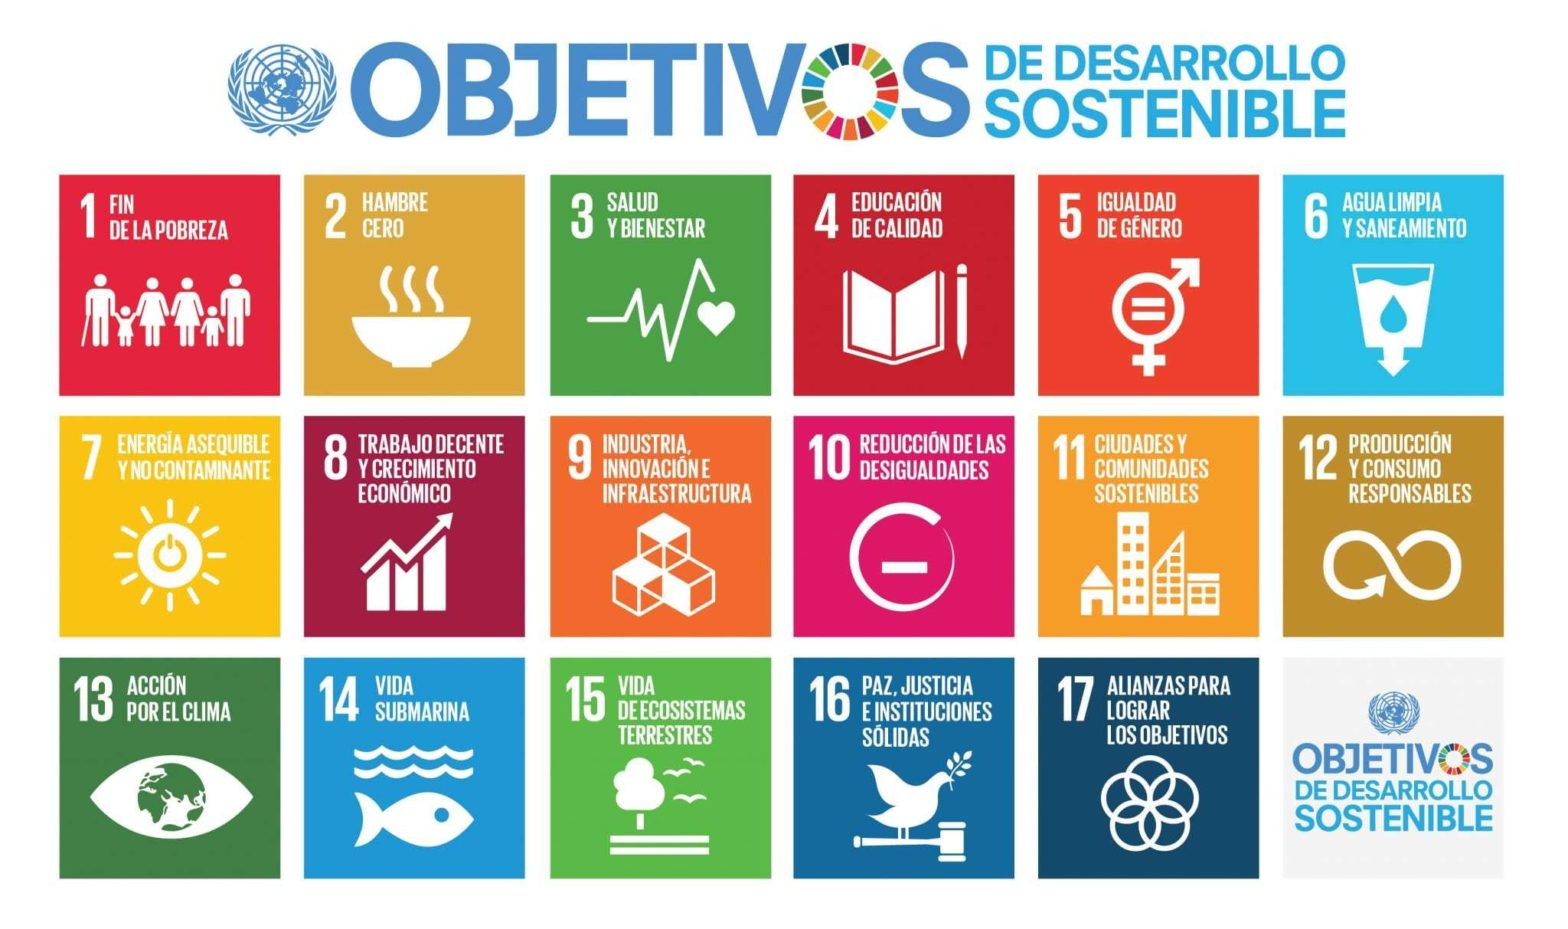
\includegraphics[scale=0.25]{images/agenda_2030.jpg}
    \caption{Objetivos de Desarrollo Sostenible (ODS) de la Agenda 2030 \cite{ODS}}
    \label{fig:ejemplo}
\end{figure}


\begin{itemize}
    \item \textbf{ODS 11: Ciudades y comunidades sostenibles.} Mejorar la movilidad urbana es fundamental para lograr ciudades más inclusivas, seguras y eficientes. Los métodos propuestos ayudan a reducir la congestión y optimizar las rutas, favoreciendo una planificación urbana basada en datos.

    \item \textbf{ODS 9: Industria, innovación e infraestructura.} El uso de herramientas avanzadas como TDA fomenta la innovación tecnológica en transporte e infraestructura, habilitando nuevos modelos de gestión urbana, control de tráfico o rutas logísticas inteligentes.
    \vspace{2cm}
    \item \textbf{ODS 3: Salud y bienestar.} Una red de movilidad más eficiente contribuye a la salud pública mediante la reducción de accidentes, tiempos de respuesta de emergencias y exposición a la contaminación. Además, el análisis de trayectorias se puede aplicar a estudios epidemiológicos.

    \item \textbf{ODS 13: Acción por el clima.} La optimización de trayectorias y flujos de transporte, ya sea terrestre o aéreo, contribuye a reducir las emisiones de gases de efecto invernadero. Las herramientas desarrolladas pueden emplearse para diseñar rutas de bajo consumo energético.
\end{itemize}

En resumen, aunque este trabajo es principalmente metodológica, sus implicaciones abarcan diversos dominios con relevancia social, científica y ambiental. La capacidad de extraer descripciones topológicas robustas de trayectorias contribuye a la toma de decisiones informadas y sostenibles en múltiples contextos de aplicación.